% --------------------------------------------------------------
% This is all preamble stuff that you don't have to worry about.
% Head down to where it says "Start here"
% --------------------------------------------------------------
 
\documentclass[12pt]{article}
 
\usepackage[margin=1in]{geometry} 
\usepackage{listings}

\usepackage{amsmath,amsthm,amssymb}
\usepackage[margin=1in]{geometry} 
\usepackage{amsmath,amsthm,amssymb}
\usepackage[spanish]{babel} %Castellanización
\usepackage[T1]{fontenc} %escribe lo del teclado
\usepackage[utf8]{inputenc} %Reconoce algunos símbolos
\usepackage{lmodern} %optimiza algunas fuentes
\usepackage{graphicx}
\graphicspath{ {images/} }
\usepackage{hyperref} % Uso de links
 
\newcommand{\N}{\mathbb{N}}
\newcommand{\Z}{\mathbb{Z}}
 
\newenvironment{theorem}[2][Theorem]{\begin{trivlist}
\item[\hskip \labelsep {\bfseries #1}\hskip \labelsep {\bfseries #2.}]}{\end{trivlist}}
\newenvironment{lemma}[2][Lemma]{\begin{trivlist}
\item[\hskip \labelsep {\bfseries #1}\hskip \labelsep {\bfseries #2.}]}{\end{trivlist}}
\newenvironment{exercise}[2][Exercise]{\begin{trivlist}
\item[\hskip \labelsep {\bfseries #1}\hskip \labelsep {\bfseries #2.}]}{\end{trivlist}}
\newenvironment{problem}[2][Problem]{\begin{trivlist}
\item[\hskip \labelsep {\bfseries #1}\hskip \labelsep {\bfseries #2.}]}{\end{trivlist}}
\newenvironment{question}[2][Question]{\begin{trivlist}
\item[\hskip \labelsep {\bfseries #1}\hskip \labelsep {\bfseries #2.}]}{\end{trivlist}}
\newenvironment{corollary}[2][Corollary]{\begin{trivlist}
\item[\hskip \labelsep {\bfseries #1}\hskip \labelsep {\bfseries #2.}]}{\end{trivlist}}

\newenvironment{solution}{\begin{proof}[Solution]}{\end{proof}}
 
\begin{document}
% --------------------------------------------------------------
%                         Start here
% --------------------------------------------------------------
\title{Tarea 9}
\author{Hanan Ronaldo Quispe Condori\\ %replace with your name
Procesamiento de Señales II}

\maketitle
\section{Realizar la simulación de un circuito RC. Determine la frecuencia de corte de su filtro (-3dB) a partir del barrido de AC del simulador. Plantee los valores de resistencia y capacitor a su criterio, pero considerando que el filtro posea una frecuencia de corte dentro del rango 1-22050 Hz, ya que se considerará como frecuencia de muestreo 44100 Hz.s}
Se uso una resistencia de valor de 1k$\Omega$ y un capacitor de $8nF$ se eligio este valor para que la frecuencia de corte este en los $20kHz$ este calculo se realizo de la siguiente manera.
\begin{equation}
    \begin{split}
        fc&=\frac{1}{2\pi RC}\\
        C&=\frac{1}{2\pi*10^3*20*10^3}F\\
        C&=7.958*10^{-9}F\approx 8nF
    \end{split}
    \label{eq:corte}
\end{equation}

El esquemático en Top Spice es el siguiente
\begin{figure}[h]
    \centering
    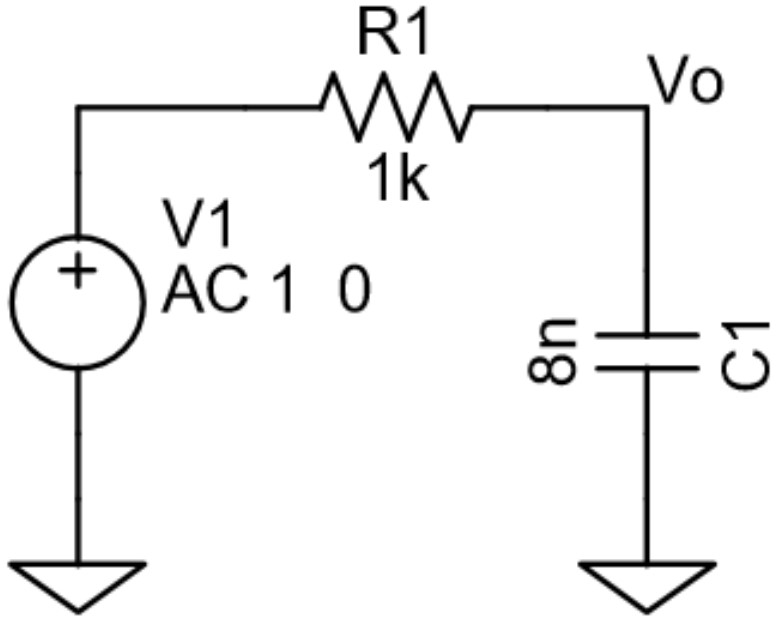
\includegraphics[width=6cm,height=4cm]{imagenes/esquematico}
    \caption{Esquemático del Circuito RC}
    \label{fig:esquematico}
\end{figure}

Los resultados de la simulación son los siguientes 

\begin{figure}[h]
    \centering
    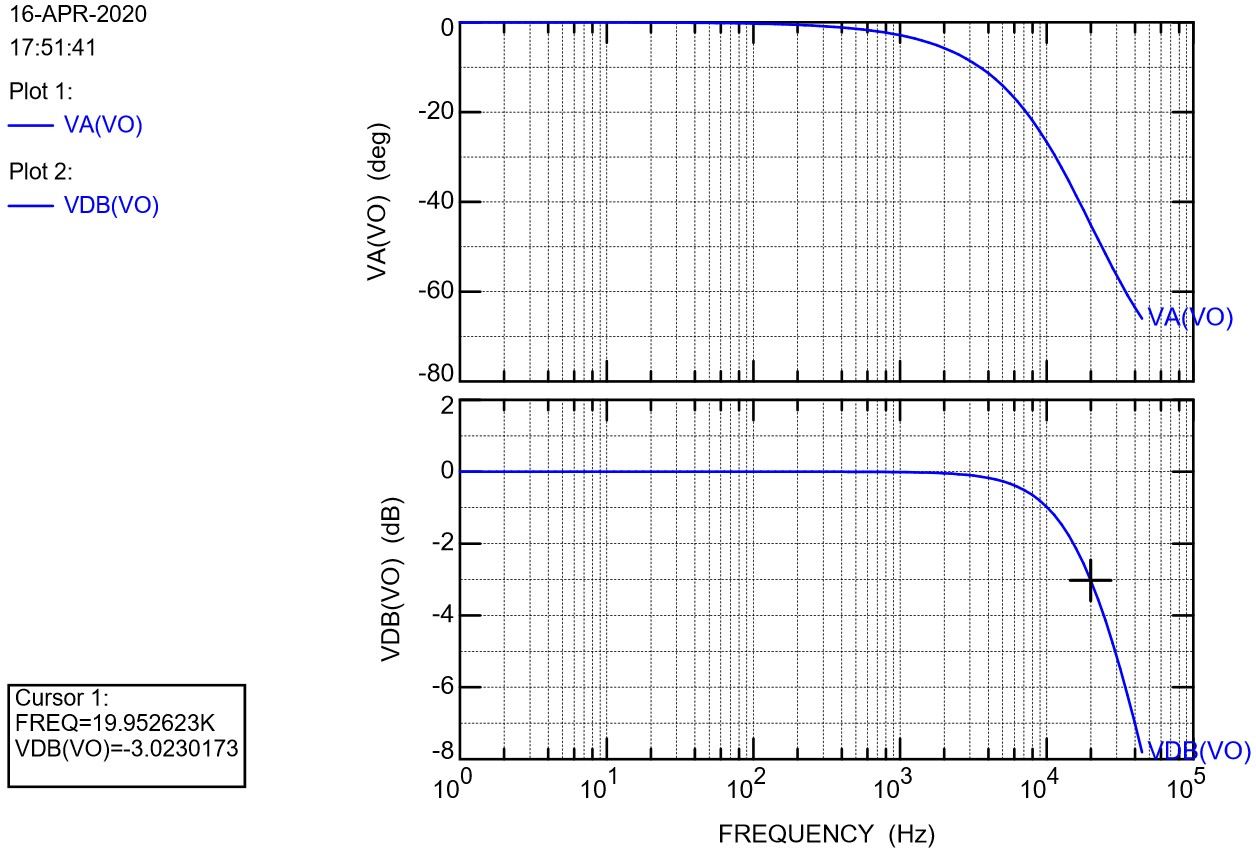
\includegraphics[width=14cm,height=11cm]{imagenes/resut1}
    \caption{Resultados Top Spice }
    \label{fig:results}
\end{figure}

De la información proporcionada por el cursor se puede observar que la frecuencia de corte de encuentra aproximadamente en el valor calculado de $20kHz$.

\section{Utilice la transformación bilineal para determinar la función de transferencia equivalente en el dominio Z del filtro. Determine la respuesta en frecuencia del filtro y compare con el resultado obtenido en el paso 2. Para ambos casos, puede utilizar el código de Matlab que se adjunta, donde viene precargado el resultado hallado en el tutorial de la tarea anterior.}

En la ultima tarea se uso la transformación bilineal para el circuito RC, el resultado fue el siguiente.

\begin{equation}
    \begin{split}
        H(z)&=\frac{1+z^{-1}}{1+\frac{2RC}{T_s}+z^{-1}*(1-\frac{2RC}{T_s})}\\
    \end{split}
    \label{eq:bilineal}
\end{equation}
Usando esta ecuación y dando valores numéricos a las variables conocidas se implementará esta función en MATLAB.

\lstinputlisting[language=Matlab]{code1.m}

Dando como resultado la siguiente gráfica. 

\begin{figure}[h]
    \centering
    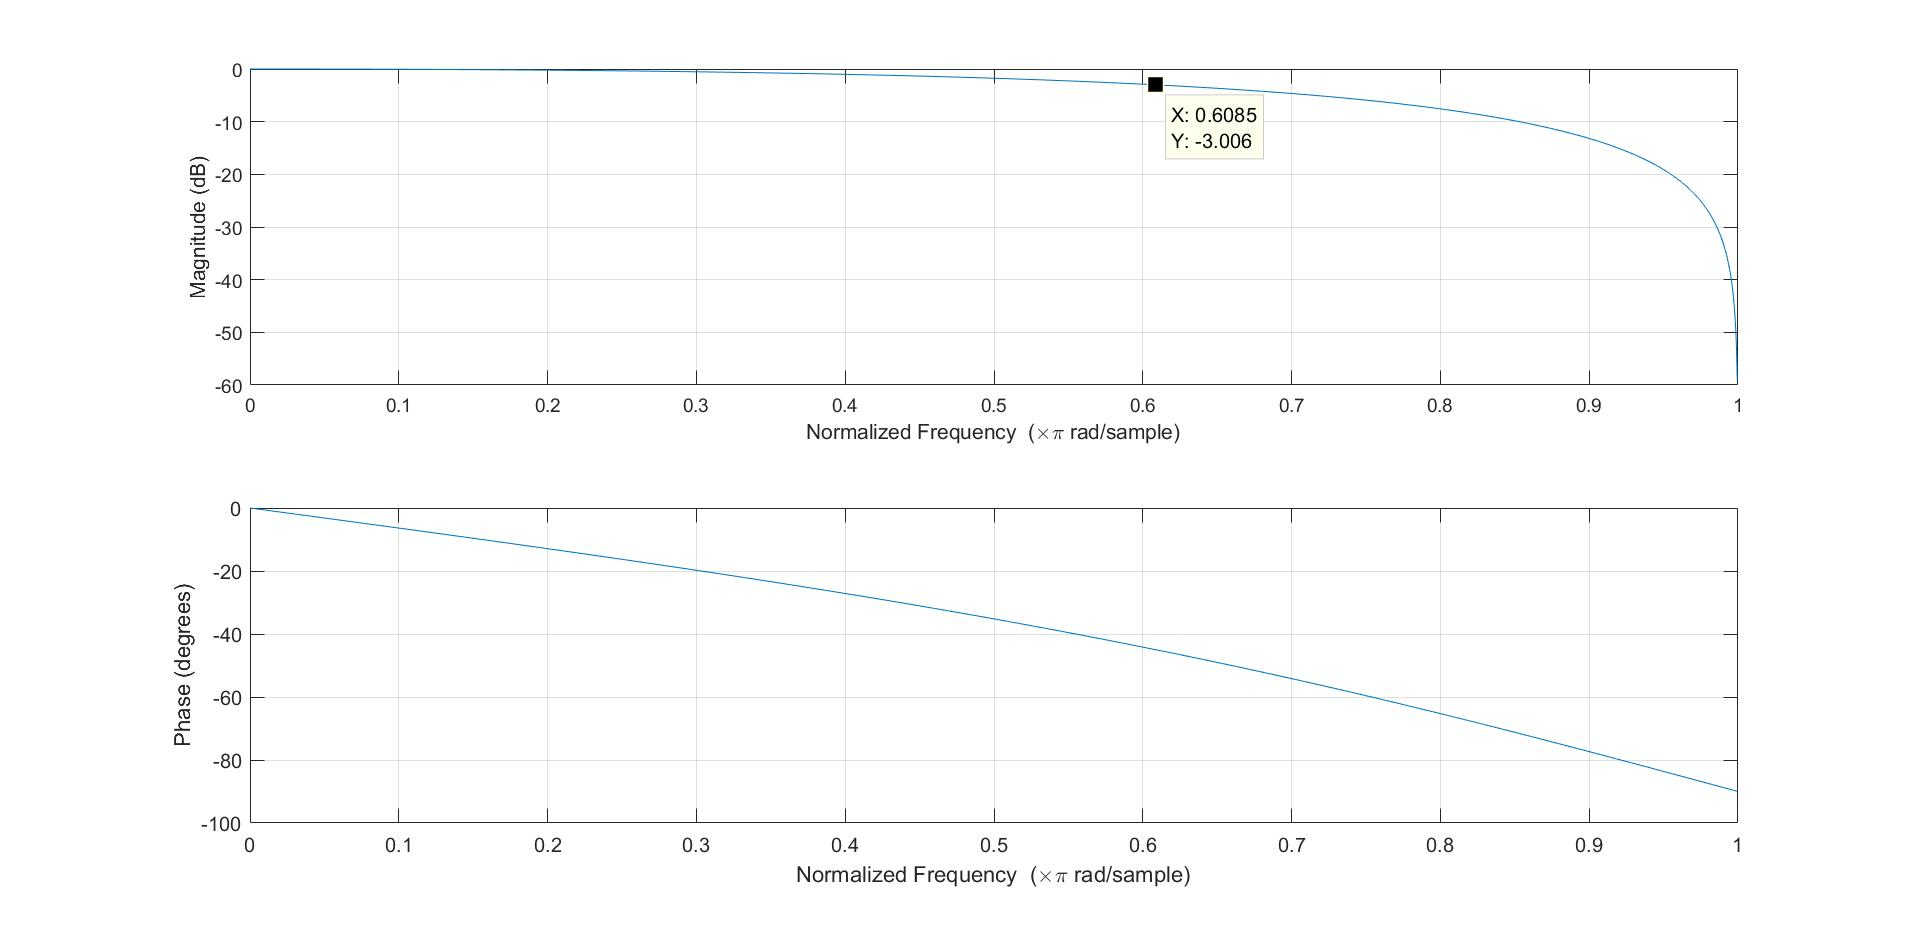
\includegraphics[width=16cm,height=11cm]{imagenes/matla}
    \caption{Resultados MATLAB }
    \label{fig:esquematico}
\end{figure}

La función $freqz$ nos da la respuesta en frecuencia normalizada cuyo valor en el punto de $-3.006dB$ corresponde a un valor de frecuencia normalizada de 0.6085 esta corresponderá a la frecuencia de corte del filtro RC.

%--------------------------------------------------------------
%     You don't have to mess with anything below this line.
% --------------------------------------------------------------
\end{document}